\begin{proof}

  \begin{enumerate}[label=$(\arabic*)$]
      \item Sia $\{E_j\}_{j=1}^n\subset \M_\phi$ ($n\geq 2$), allora $\forall A\in \P(X)$ si ha
      \[\phi(A)\overset{(i)}=\underline{\phi(A\cap E_1)}+\phi(A\cap E_1^c)\overset{(ii)}=\phi(A\cap E_1\cap E_2)+\underbrace{\phi(A\cap E_1 \cap E_2^c)+\phi(A\cap E_1^c)}_{(\dagger)}\]
      Siccome $E_1, E_2\in \M_\phi$, spezzo prima su $E_1\ (i)$ e poi su $E_2\ (ii)$. Ora applichiamo la $\sigma$-subadditività a $(\dagger)$ e otteniamo
      \[\begin{aligned}(\dagger) & \geq  \phi\left( (A\cap E_1 \cap E_2^c)\cup (A\cap E_1^c) \right)= \varphi(A\cap[(E_1\cap E_2^c)\cup E_1^c]) =\\&= \phi(A\cap [(\underbrace{E_1\cup E_1^c}_X)\cap (E_1^c\cup E_2^c)])= \phi(A\cap(E_1\cap E_2)^c)\end{aligned}.\]
      Di conseguenza otteniamo che $\phi(A)\geq \phi(A\cap (E_1\cap E_2))+\phi(A\cap (E_1\cap E_2)
      ^c)$ e iterando il procedimento si ottiene la tesi.
      \item Iniziamo provando $(*)$. Sia $A\in \P(X)$, allora
      \[\phi(A)=\phi(A\cap E_1)+\phi(A\cap E_1^c)=\phi(A\cap E_1)+\phi(A\cap \underline{E_1^c\cap E_2})+ \phi(A\cap E_1^c\cap E_2^c)=\]
      Siccome $E_1\cap E_2=\varnothing$, $E_2\subset E_1^c \implies E_1^c\cap E_2=E_2$
      \[=\phi(A\cap E_1)+\phi(A\cap E_2)+\phi(A\cap (E_1\cup E_2)^c).\]
      Iterando questo argomento otteniamo quindi 
      \[\phi(A)=\sum_{j=1}^n\phi(A\cap E_j)+\phi\left( A\cap \left[ \bigcup_{j=1}^nE_j \right]^c \right)\overset{(\ddagger)}\geq \sum_{j=1}^n\phi(A\cap E_j)+\phi(A\cap S^c).\]
      $(\ddagger)$ in quanto $\bigcup_{j=1}^n E_j\subset S\implies \left[ \bigcup_{j=1}^n E_j\right]^c \supset S^c \implies A\cap \left[ \bigcup_{j=1}^n E_j\right]^c \supset A\cap S^c$ quindi per la monotonia di $\phi$, si ha $\phi\left( A\cap \left[ \bigcup_{j=1}^n E_j\right]^c\right)\geq \phi(A\cap S^c)$. 

      Poiché gli addendi della sommatoria sono non negativi, il limite delle somme parziali esiste. Passando quindi al limite per $n\to +\infty$ si ha 
      \[\phi(A)\geq \sum_{j}\phi(A\cap E_j)+\phi(A\cap S^c)\]
      E questo conclude la dimostrazione di $(*)$. Ora proviamo che $S\in \M_\phi$. Sia $A\in \P(X)$. Inizialmente osserviamo che $A\cap S = A\cap \left( \bigcup_{j}E_j\right) = \bigcup_j(A\cap E_j)$. Di conseguenza per la $\sigma$ subadditività di $\phi$ 
      \[\phi(A\cap S)+\phi(A\cap S^c)\leq \sum_{j} \phi(A\cap E_j)+\phi(A\cap S^c)\overset{(\ast)}{\leq} \phi(A)\]
      \item Usando $(\ast)$ con $A=S$ 
      \[\phi\left( \bigcup_i E_i\right) = \phi(S) \geq \sum_j\underset{\bigcup_iE_i\cap E_j=E_j}{\phi(\underbrace{S\cap E_j})}+\phi(\underbrace{S\cap S^c}_{\varnothing}) = \sum_j\phi(E_j)\overset{(\bullet)}{\geq} \phi\left( \bigcup _jE_j \right).\]
      $(\bullet)$ per la $\sigma$-subadditività.
      Di conseguenza $\phi\left( \bigcup_jE_j \right)= \sum _j\phi(E_j)$.
  \end{enumerate}
  
\end{proof}


\begin{remark}\label{oss: unione in mphi} Sia data una misura esterna $\varphi$ su $X$ e sia $\left\{E_{j}\right\}$ una famiglia numerabile di insiemi misurabili. Poniamo $E_{1}^{*}:=E_{1}$ e
\[
E_{n}^{*}:=E_{n}\setminus \bigcup_{j=1}^{n-1} E_{j} \quad(n=2,3, \ldots) .
\]
Allora $\left\{E_{j}^{*}\right\}$ è una famiglia numerabile di insiemi misurabili a-due-a-due disgiunti e si ha
\[
\bigcup_{j=1}^{n} E_{j}^{*}=\bigcup_{j=1}^{n} E_{j}\ \ (\text {per ogni } n), \quad \bigcup_{j} E_{j}^{*}=\bigcup_{j} E_{j} \text {. }
\]
In particolare, ricordando il punto (4) di Teorema \ref{thm: proprietà misurabili}, si ha $\bigcup_{j} E_{j} \in \mc{M}_{\varphi}$.
\end{remark}
\begin{definition} \label{def: sigma-algebra} Una famiglia non vuota $\Sigma \subset \P(X)$ è detta "$\sigma$-algebra (in $X$)" se gode delle seguenti proprietà:
\begin{enumerate}[label=$(\roman*)$]
  \item Se $E \in \Sigma$, allora $E^{c} \in \Sigma$;
  \item $S e\left\{E_{j}\right\}$ è una famiglia numerabile di insiemi di $\Sigma$, si ha $\cup_{j} E_{j} \in \Sigma$.
\end{enumerate}
\end{definition}
\begin{remark}In Definizione \ref{def: sigma-algebra} l'assioma $(ii)$ può venir sostituito da
\begin{enumerate}[label=$(\roman*^*$), start=2]
  \item Se $\left\{E_{j}\right\}$ è una famiglia numerabile di insiemi di $\Sigma$, si ha $\cap_{j} E_{j} \in \Sigma$.
\end{enumerate}
\end{remark}
\begin{example}Sia $X$ un qualsiasi insieme. Allora $\P(X)$ e $\{\varnothing, X\}$ sono entrambe $\sigma$-algebre in $X$. Se $\Sigma$ è una qualsiasi $\sigma$-algebra in $X$, si ha $\{\varnothing, X\} \subset \Sigma \subset \P(X)$.
\end{example}

\begin{example}$\Sigma:=\left\{E \in 2^{[0,1]} \mid \#(E) \leq \aleph_{0}\right.$ oppure $\left.\#\left(E^{c}\right) \leq \aleph_{0}\right\}$ è una $\sigma$-algebra.
\end{example}
\begin{example}La famiglia $\Sigma:=\left\{E \in \P(\N) \mid \#(E)<\infty\right.$ oppure $\left.\#\left(E^{c}\right)<\infty\right\}$ è $c$-chiusa ma non è chiusa rispetto all'unione numerabile. Quindi $\Sigma$ non è una $\sigma$-algebra.
\end{example}
Per Teorema \ref{thm: proprietà misurabili} e Osservazione \ref{oss: unione in mphi}, vale quindi il seguente risultato.

\begin{proposition}[$\circ$]\label{prop: misurabili sigma-algebra} Se $\varphi$ è una misura esterna su $X$, allora $\mc{M}_{\varphi}$ è una $\sigma$-algebra.
\end{proposition}
\begin{proof}
  Verifichiamo gli assiomi di $\sigma$-algebra:
  \begin{enumerate}[label=$\roman*)$]
      \item [\textbullet] \textbf{Non vuota} in quanto per il Teorema \ref{thm: proprietà misurabili}.(2), $\varnothing, X \in \M_\phi$;
      \item \textbf{c-chiusa} per il Teorema \ref{thm: proprietà misurabili}.(1);
      \item \textbf{Stabile per unione numerabile}. Per il Teorema \ref{thm: proprietà misurabili}.(4), $M_\phi$ è chiusa per unione numerabile di insiemi disgiunti. Proviamo che chò vale anche se gli insiemi non sono a due a due disgiunti: Sia $\{E_j\}_j\subset M_\phi$ una famiglia finita. Poniamo $E_1^*=E_1$ e $\forall k\geq 2$ definiamo $E_k^*:=E_k\setminus \bigcup_{j=1}^{k-1}E_j = E_k\cap \left( \bigcup_{j=1}^{k-1}E_j \right)^c$, ovvero tutti gli elementi che stanno in $E_k$ ma non nei precedenti componenti della famiglia. Per il Teorema \ref{thm: proprietà misurabili}, si ha che $\forall k,\ E_k\in M_\phi$, quindi possiamo affermare la seguente equivalenza, in cui il membro di destra soddisfa le ipotesi del Teorema \ref{thm: proprietà misurabili}.(4), ovvero è unione di insiemi disgiunti.
      \[\bigcup_{k=1}^NE_k=\bigcup_{k=1}^NE_k^*.\]
      Poiché l'uguaglianza rimane verificata anche per $N\to +\infty$ (passando all'unione arbitraria numerabile), si ha che per il Teorema \ref{thm: proprietà misurabili}.(4), $\bigcup_{j} E_j= \bigcup_{j} E_j^*\in M_\phi$.
  \end{enumerate}
\end{proof}

\begin{shadedTheorem}[$**$]\label{thm: continuità misure esterne}
  Se $\phi$ è una misura esterna si $X$, valgono le seguenti proprietà:
  \begin{enumerate}[label=$(\arabic*)$]
      \item (Continuità dal basso) Se $\{E_j\}_j$ è una famiglia numerabile e crescente di insiemi misurabili, si ha $\phi\left(\bigcup_jE_j\right) = \lim_j\phi(E_j)$;
      \item (Continuità dall'alto) Se $\{E_j\}_j$ è una famiglia numerabile e decrescente di insiemi misurabili con $\phi(E_1)<\infty$,  si ha $\phi\left(\bigcap_jE_j\right) = \lim_j\phi(E_j)$;
  \end{enumerate}
\end{shadedTheorem}

\begin{proof}~
  \begin{enumerate}[label=$(\arabic*)$]
      \item (Continuità dal basso) Poniamo $E_1^*=E_1$ e $\forall j\geq 2$ definiamo $E_j^*:=E_j\setminus \bigcup_{k=1}^{j-1}E_k = E_j \setminus E_{j-1}\in M_\phi$. Osserviamo che $(\dagger)\ \bigcup_{j=1}^nE_j^*=\bigcup_{j=1}^nE_j=E_n$ quindi $\bigcup_jE_j^*=\bigcup_jE_j$.
      \[\implies \phi\left( \bigcup_jE_j\right)=\phi\left( \bigcup_jE_j^* \right) \overset{\sigma\text{-add}}{=} \sum_j\phi(E_j)=\lim_{n\to+\infty}\sum_{j=1}^n\phi(E_j^*) =\]
      per definizione di serie. È possibile applicare la $\sigma$-additività poiché gli insiemi $E_j^*$ sono disgiunti.
      \[=\lim_{n\to+\infty}\phi\left( \bigcup_{j=1}^nE_j^* \right) \overset{(\dagger)}=\lim_{n\to+\infty}\phi(E_n)\]
      \item (Continuità dall'alto) Poniamo $\forall j,\ F_j=E_1\setminus E_j = E_1\cap E_j^c\in \M\phi$. Osserviamo inoltre che $E_{j}\supset E_{j+1} \implies E_j^c\subset E_{j+1}^c \implies E_1\cap E_j^c\subset E_1\cap E_{j+1}^c$ da cui $F_j\subset F_j+1$, ovvero $\{F_j\}_j$ soddisfa le ipotesi di $(1)$, per cui $(\triangle)\ \phi\left( \bigcup_jF_j \right) = \lim_j\phi(F_j)$. Osserviamo ora che
      \[\tag{\textbullet}\phi(F_j)=\phi(E_1\setminus E_j)=\phi(E_1)-\phi(E_j)\]
      in quanto per il buon spezzamento ($E_j\in M_\phi, E_j\subset E_1$)
      \[\phi(E_1)=\phi(E_1\cap E_j)=\phi(E_1\setminus E_j)=\phi(E_j)+\phi(E_1\setminus E_j)\]
      Allora poiché $\phi(E_1)<\infty$, $\phi(F_j)=\phi(E_1)-\phi(E_j)<+\infty$. Abbiamo quindi 
      \[\lim_{j\to+\infty}\phi(F_j)=\phi(E_1)-\lim_{j\to+\infty}\phi(E_j)\tag{$*$}\]
      Analizziamo ora $\phi\left(\bigcup_jF_j\right)$
      \[\begin{aligned}
          \phi\left( \bigcup\nolimits_jF_j \right)&=\phi\left( \bigcup\nolimits_j(E_1\cap E_j^c) \right)= \phi\left(E_1\cap \left( \bigcup\nolimits_jE_j^c \right)\right) \overset{De\ M.}{=} \phi\left( E_1\cap\left( \bigcap\nolimits_jE_j\right)^c \right) =\\&= \phi\left( E_1\setminus \left( \bigcap\nolimits_jE_j \right) \right) \overset{\text{come (\textbullet)}}{=\dots=} \phi(E_1)-\phi\left( \bigcap\nolimits_jE_j \right) 
      \end{aligned}\]
      Abbiamo quindi provato che \[\phi\left( \bigcup\nolimits_jF_j \right) = \phi(E_1)-\phi\left(\bigcap\nolimits_jE_j\right)\tag{$**$}\]
      Sostituendo quindi $(*)$ e $(**)$ in $(\triangle)$ otteniamo 
      \[\cancel{\phi(E_1)}-\phi\left( \bigcap\nolimits_jE_j \right)=\cancel{\phi(E_1)}-\lim_{j\to+\infty}\phi(E_j)\]
      \[\implies\quad \phi\left( \bigcap\nolimits_jE_j \right)=\lim_{j\to+\infty}\phi(E_j)\]
  \end{enumerate}
\end{proof}

\begin{remark} Se in (2) di Teorema \ref{thm: continuità misure esterne} non si assume l'ipotesi $\varphi\left(E_{1}\right)<\infty$, la tesi può fallire. Per esempio, se $X:=\N$ con $\varphi(E):=\#(E)$, possiamo considerare la famiglia degli $E_{j}:=\{j, j+1, \ldots\} \in \mc{M}_{\varphi}=\P(X)$. In tal caso si ha $\bigcap_{j} E_{j}=\varnothing$ e quindi $\varphi\left(\bigcap_{j} E_{j}\right)=0$, mentre $\varphi\left(E_{j}\right)=\infty$ per ogni $j$.
\end{remark}

\section{Misure esterne metriche, Boreliane, Borel-regolari, di Radón}
\begin{definition}
  Una misura esterna su uno spazio metrico $(X, d)$ è detta "di Carathéodory" (oppure "metrica") se
  \[
  \varphi(A \cup B)=\varphi(A)+\varphi(B)
  \]
  
  per ogni coppia di insiemi $A, B \in \P(X)$ tale che
  
  \[
  \operatorname{dist}(A, B):=\inf \{d(a, b) \mid a \in A, b \in B\}>0
  \]
\end{definition}


\begin{shadedTheorem}[$***$| \textsc{Carathéodory}] \label{CARATHEODORY} Sia $\varphi$ una misura esterna di Carathéodory su uno spazio metrico $(X, d)$. Allora ogni sottoinsieme chiuso di $X$ è misurabile.
\end{shadedTheorem}
\begin{proof}
  Sia $C\subset X$ chiuso, $A\in \P(X)$ chiuso. Vogliamo dimostrare il buon spezzamento, ovvero 
  $\phi(A)\geq \phi(A\cap C)+\phi(A\cap C^c)$ (poiché il $\leq$ è garantito dalla $\sigma$-subadditività). Se $\phi(A)=+\infty$, la tesi è banale; sia quindi $A$ tale che $\phi(A)<+\infty$. Per ogni $h\in \N^*$ poniamo \[C_h:=\left\{x\in X\, \bigg|\, \operatorname{dist}(\{x\}, C)\leq \frac{1}{h}\right\}\]
  \begin{figure}[ht]
      \centering
      \begin{tikzpicture}
      \draw (0,0) ellipse (2 and 1);
      \node at (1.8,0.8) {$A$};
      \draw (-1.5,0) circle (1.8);
      \node at (-0.1,1.5) {$C_h$};
      \draw[dotted] (-1.5,0) circle (1.5);
      \draw[dotted] (-1.5,0) circle (1.3);
      \draw[dotted] (-1.5,0) circle (1.2);
      \draw[dotted] (-1.5,0) circle (1.1);
      \draw[dotted] (-1.5,0) circle (1.05);
      \draw (-1.5,0) circle (1);
      \node at (-0.6,0.8) {$C$};
      \draw[-to] (-0.5,0) -- node[above]{$\frac{1}{h}$} (0.3,0);
      \draw[to-] (-0.5,0) -- (0.3,0);
      \draw[pattern=north west lines, pattern color=blue] (-1,0.87) arc
      [
          start angle=120,
          end angle=240,
          x radius=2cm,
          y radius =1cm
      ]--(-1,-0.87) arc (-60:60:1);
      \node at (-1.3,0) {$A\cap C$};   

      \draw[pattern=north west lines, pattern color=red] (0,-1) arc
      [
          start angle=-90,
          end angle=90,
          x radius=2cm,
          y radius =1cm
      ]--(0,1) arc (33.75:-33.75:1.8);
      \node at (1.1,0) {$A\cap C_h^c$};  

  \end{tikzpicture}
  \caption{Gli insiemi utilizzati per la dimostrazione}
  \end{figure}
  e osserviamo che è chiuso poiché controimmagine di un chiuso $[0, \frac{1}{h}]$ mediante la funzione distanza che è continua. 
  Segue quindi che \[(i)\ \operatorname{dist}(A\cap C, A\cap C^c_h)=\frac{1}{h}\quad e \quad (ii)\ {A\cap C}\cup (A\cap C^c_h)\subset A\]
  quindi per $(ii)$ e monotonia di $\phi$ si ha 
      \[\phi(A)\geq \phi((A\cap C)\cup (A\cap C_h^c))=\phi(A\cap C)+\phi(A\cap C_h^c)\]
  per la metricità di $\phi$. Per ottenere la tesi è quindi sufficiente provare che 
  \[\lim_{n\to+\infty}\phi(A\cap C_h^c)=\phi(A\cap C^c).\]
  Per prima cosa notiamo che il limite esiste per monotonia. Osserviamo ora che 
  \[\begin{aligned}
      C_h & = 
          \left\{x\in X\,|\,\operatorname{dist}(\{x\},X)=0\right\}\sqcup\left\{x\in X\,\bigg|\,\operatorname{dist}(\{x,C\})\in \left]0, \frac{1}{h}\right]\right\} =\\
          & = C \sqcup \bigcup_{j=h}^{+\infty}\underbrace{\left\{x\in X\,\bigg|\, \operatorname{dist}(\{x\},X)\in \left]\frac{1}{j+1}, \frac{1}{j}\right]\right\}}_{S_j}
  \end{aligned}\] 
  
  \[\Harr\ C=C_h\setminus \bigcup_{j=h}^{+\infty}S_j=C_h\cap \bigg( \bigcup_{j=h}^{+\infty} S_j \bigg)^c,\]
  quindi che per le leggi di De Morgan l'identità precedente può essere riscritta come 
  \[C_h^c\subset C^c=C^c_h\cup \bigcup_{j=h}^{+\infty}S_j\quad \implies \quad A\cap C_h^c\subset A\cap C^c=(A\cap C_h^c) \cup \bigg(\bigcup_{j=n}^{+\infty}(A\cap S_j)\bigg)\]
  di conseguenza per monotonia di $\phi$ e per la $\sigma$-subadditività
  \[\phi(A\cap C_h^c)\leq \phi(A\cap C^c) = \phi\bigg((A\cap C^c_h)\cup \bigg(\bigcup_{j=h}^{+\infty}(A\cap S_j)\bigg)\bigg)\leq \phi(A\cap C^c_h)+\sum _{j=h}^{+\infty} \phi(A\cap S_j)\]
  Se ora proviamo che (\textbullet) $\lim\limits_{h\to +\infty}\sum_{j=h}^{+\infty}\phi(A\cap S_j)=0$, otteniamo che $\phi(A\cap C^c_\infty)\leq \phi(A\cap C^c)\leq \phi(A\cap C_\infty^c)$, ovvero che le due quantità sono uguali.

  Poiché (\textbullet) è il resto $h$-esimo della serie $\sum_j\phi(A\cap S_j)$, equivale a dire che la suddetta serie converge. Poiché si tratta di una serie a termini positivi, la successione delle somme parziali è crescente quindi il limite esiste. Per provare la convergenza della serie è quindi sufficiente provare che la successione delle somme parziali è limitata. Osserviamo che

  \[\sum_{j=1}^N\phi(A\cap S_j)=\sum_{\substack{j\leq N\\j \text{ dispari}}}\phi(A\cap S_j)+\sum_{\substack{j\leq N\\j \text{ pari}}}\phi(A\cap S_j)\]

  poichié $\operatorname{dist}(S_j, S_k)>0\ \forall j,k $ entrambi pari o entrambi dispari e $\phi$ è metrica 
  \[\phi(A\cap S_1)+\phi(A\cap S_3)=\phi((A\cap S_2)\cup (A\cap S_3))\]
  quindi generalizzando
  \[\sum_{j=1}^N\phi(A\cap S_j)=\phi\bigg(\underbrace{\!\!\!\!\bigcup_{\substack{j\leq N\\j \text{ dispari}}}\!\!\!A\cap S_j}_{\subset A}\bigg)+\phi\bigg(\underbrace{\!\!\bigcup_{\substack{j\leq N\\j \text{ pari}}}\!\!\!A\cap S_j}_{\subset A}\bigg)\overset{monot.}{\leq} 2\phi(A)<+\infty\]
  per ipotesi iniziale. Di conseguenza per il teorema di esistenza del limite per successioni monotone, la serie converge. 
\end{proof}
\begin{remark}
  Si può provare che vale anche il "viceversa" di Teorema \ref{CARATHEODORY}: Se $\varphi$ è una misura esterna su uno spazio metrico $(X, d)$ e se ogni sottoinsieme chiuso di $X$ è misurabile, allora $\varphi$ è di Carathéodory ([12, Theorem 1.7]).
\end{remark}

\begin{proposition}[$*$]\label{prop: sigma algbra generata}Sia dato $\mc{I} \subset \P(X)$ e indichiamo con $\mc{A}_{\mc{I}}$ la famiglia delle $\sigma$-algebre in $X$ contenti $\mc{I}$. Allora
\[
\Sigma(\mc{I}):=\bigcap_{\Sigma \in \mc{A}_{\mc{I}}} \Sigma
\]
è una $\sigma$-algebra in $X$, detta "la $\sigma$-algebra generata da $\mc{I} "$. Se $\mc{I}$ è una $\sigma$-algebra allora $\Sigma(\mc{I})=\mc{I}$. Inoltre la mappa $\mc{I} \mapsto \Sigma(\mc{I})$ è monotona crescente, i.e., $\Sigma\left(\mc{I}_{1}\right) \subset \Sigma\left(\mc{I}_{2}\right)$ ogni volta che $\mc{I}_{1} \subset \mc{I}_{2} \subset \P(X)$.
\end{proposition}
\begin{proof}~
  \begin{itemize}
      \item \underline{\bf$\Sigma(I)\in\mc{A_I}$:} Osserviamo prima di tutto che banalmente $\mc{I}\in \Sigma(\mc{I})$, in quanto $\forall \Sigma \in \mc{A_I}, \mc{I}\subset \Sigma$. Verifichiamo ora gli assiomi di $\sigma$-algebra:
      \begin{enumerate}[label=(\arabic*)]
          \item Sia $E\in \Sigma(\mc{I})=\bigcap_{\Sigma\in\mc{A_I}}\Sigma$. Allora $\forall \Sigma\in \mc{A_I}$, $E\in \Sigma$ e poiché $\Sigma$ è una $\sigma$-algebra, $E^c\in \Sigma$. Di conseguenza $E^c\in \Sigma(\mc{I})$.
          \item Analogamente, si ha la chiusura rispetto all'unione numerabile: Sia $\{E_j\}_j\subset \Sigma(\mc{I})=\bigcap_{\Sigma\in\mc{A_I}}\Sigma$ numerabile. Allora $\forall \Sigma\in \mc{A_I}, \forall j$, $E_j\in \Sigma$ e poiché $\Sigma$ è una $\sigma$-algebra, $\bigcup_{j}E_j\in \Sigma$. Di conseguenza $\bigcup_jE_j\in \Sigma(\mc{I})$
      \end{enumerate} 
      Siccome $\Sigma(\mc{I})$ è una $\sigma$-algebra e contiene $\mc{I}$, allora $\Sigma(\mc{I})\in \mc{A_I}$.
      \item \textbf{\underline{Stabilità}}: Sia $\mc{I}$ una $\sigma$-algebra, proviamo che  $\Sigma(\mc{I})=\mc{I}$. Ovviamente $\mc{I}\in \mc{A_I}$, quindi (per il punto precedente)
      \[\Sigma(\mc{I})=\bigcap_{\Sigma\in\mc{A_I}}\Sigma\subset \mc{I}\subset \Sigma(I)\implies \Sigma(\mc{I})=\mc{I}\]
      \item \underline{\textbf{Monotonia:}} Siano $\mc{I}_1, \mc{I}_2\subset \P(X)$ con $\mc{I}_1\subset\mc{I}_2$. Si ha subito che $\mc{A}_{\mc{I}_1}\supset \mc{A}_{\mc{I}_2}$ poiché $\Sigma\in \mc{A}_{\mc{I}_2} \Rarr \mc{I}_2\subset \Sigma \Rarr \mc{I}_1 \subset \mc{I}_2 \subset \Sigma \Rarr \Sigma\in \mc{A}_{\mc{I}_1}$. Segue quindi che $\bigcap_{\Sigma\in \mc{A}_{\mc{I}_1}}\Sigma \subset \bigcap_{\mc{A}_{\mc{I}_2}}\Sigma$ in quanto nel primo caso stiamo intersecando gli stessi insiemi che ci sono nel secondo più degli altri, che vanno quindi a \say{restringere} l'intersezione. Di conseguenza $\Sigma(\mc{I}_1)\subset \Sigma(\mc{I}_2)$.\qedhere
  \end{itemize}
\end{proof}

\begin{proposition}[$**$]\label{prop: 1.3 boreliani} Sia $X$ uno spazio topologico e indichiamo con $\mc{K}, \mc{F}$ e $\mc{G}$, rispettivamente, la famiglia degli insiemi compatti, la famiglia degli insiemi chiusi e la famiglia degli insiemi aperti di $X$. Allora:
  \begin{enumerate}
    \item Si ha $\Sigma(\mc{F})=\Sigma(\mc{G})$;

    \item Se $X$ è uno spazio di Hausdorff, vale l'inclusione $\Sigma(\mc{K}) \subset \Sigma(\mc{F})$;

    \item Se $(X, d)$ è uno spazio metrico separabile, si ha $\Sigma(\mc{K})=\Sigma(\mc{G})$ (dimostrato nel caso particolare dello spazio Euclideo; per una trattazione del caso generale si può vedere [13])\footnote{NdR. In realtà questa proprietà non è vera in generale, in quanto sono possibili controesempi in spazi metrici separabili di dimensione infinita. Tuttavia rimane valida nel caso dello spazio euclideo, quindi nei casi presi in esame in questo corso è vera. }.
  \end{enumerate}
\end{proposition}
\begin{proof}~
  \begin{enumerate}[label=$(\arabic*)$]
      \item Per la Proposizione \ref{prop: sigma algbra generata}, $\mc{F}\in \Sigma(\mc{F})$. Allora $\forall G\in \mc{G}$, si ha $G^c\in \mc{F}\subset \Sigma(\mc{F})$. Di conseguenza per l'assioma di c-chiusura, $G\in \Sigma(\mc{F})$. Per l'arbitrarietà gi $G$, $\mc{G}\subset \Sigma(\mc{F})$. Segue quindi per monotonia che $\Sigma(\mc{G})\subset \Sigma(\Sigma(\mc{F}))=\Sigma(\mc{F})$ per stabilità. Analogamente si dimostra che $\Sigma(\mc{F})\subset \Sigma(\mc{G})$. Segue quindi dalla doppia inclusione che  $\Sigma(\mc{F}) = \Sigma(\mc{G})$.
      \item Poiché $X$ è uno spazio di Hausdorff, si ha che $\mc{K}\subset \mc{F}$, quindi $\Sigma(\mc{K})\subset \Sigma(\mc{F})$ per monotonia.
      \item {[Dimostrazione in $\R^n$, facilmente adattabile]} Poiché $X$ è uno spazio metrico, allora $X$ è di Hausdorff, quindi $\mc{K}\subset \mc{F}$, per cui $\Sigma(\mc{K})\subset \Sigma(\mc{F})=\Sigma(\mc{G})$. Proviamo che $\Sigma(\mc{G})\subset \Sigma(\mc{K})$. È quindi sufficiente provare che $\mc{G}\subset \Sigma (\mc{K})$. Sia quindi $G\in \mc{G}$ qualsiasi, proviamo che $G\in \Sigma(\mc{K})$.
      
      \textbf{Notazione:} Indichiamo con $\mc{B}=\{\overline{B_r(Q)}\,|\,r\in \Q^+, Q\in \Q^n, \overline{B_r(Q)}\subset G\}$ la famiglia delle palle chiuse di raggio e centro razionali contenute in $G$. Osserviamo che è possibile definire una mappa iniettiva  $\mc{B}\ni \overline{B_r(Q)}\mapsto (r,Q)\in\Q^{n+1}$, per cui $\mc{B}$ è numerabile. 

      Proviamo quindi che $\bigcup_{D\in \mc{B}}D=G$. Per costruzione è banale che $\bigcup_{D\in \mc{B}}D\subset G$. Sia ora $x\in G$, proviamo che $\exists D\in \mc{B}:\ x\in D$. Sia $R>0$ tale che $B_r(x)\subset G$. Consideriamo $r\in \Q : 0<r<\frac{R}{2}$. Sia inoltre $Q\in \Q$ tale che $\|Q-x\|\leq r$, allora $x\in \overline{B_r(Q)}$. Rimane quindi da provare che $\overline{B_r(Q)}\in\mc{B}$, ovvero che $\overline{B_r(Q)}\subset G$, o meglio che $\overline{B_r(Q)}\subset B_R(x)$. Sia quindi $y\in B_R(Q)$ qualsiasi, per la disuguaglianza triangolare si ha che 
      \[\|y-x\|\leq \underbrace{\|y-Q\|}_{\leq r}+\underbrace{\|Q-x\|}_{\leq r}\leq 2r <R\quad \implies \overline{B_r(Q)}\in \mc{B}\]
      Abbiamo così provato che $G=\bigcup_{D\in \mc{B}}D$. Poiché $D\in \mc{K}$, e $\mc{B}$ è numerabile, segue per stabilità rispetto all'unione numerabile che $G\in \Sigma(\mc{K})$.
  \end{enumerate}
\end{proof}


\begin{remark}In uno spazio topologico che non sia metrico e separabile può effettivamente accadere che $\Sigma(\mc{K}) \neq \Sigma(\mc{F})=\Sigma(\mc{G})$. Si consideri per esempio $[0,1]$ con la topologia discreta e cioè $\mc{G}:=2^{[0,1]}$. Osserviamo che $\mc{K}$ coincide con la famiglia dei sottoinsiemi finiti di $[0,1]$. Se consideriamo la $\sigma$-algebra

$$
\Sigma_{0}:=\left\{E \in 2^{[0,1]} \mid \#(E) \leq \aleph_{0} \text { oppure } \#\left(E^{c}\right) \leq \aleph_{0}\right\}
$$

introdotta in Esempio 1.6, si ha $\Sigma(\mc{K}) \subset \Sigma_{0} \subset 2^{[0,1]}$. Inoltre, evidentemente, vale $\Sigma_{0} \neq$ $2^{[0,1]}=\mc{G}=\Sigma(\mc{G})$.
\end{remark}
\begin{definition}
  Siano $X$ uno spazio topologico, $\varphi$ una misura esterna su $X$ e $\mc{M}_{\varphi}$ la $\sigma$-algebra degli insiemi misurabili rispetto a $\varphi$. Allora:
  \begin{enumerate}[label=$(\roman*)$]
    \item La $\sigma$-algebra $\Sigma(\mc{F})=\Sigma(\mc{G})$ viene indicata con $\mc{B}(X)$ e $i$ suoi elementi sono detti "insiemi Boreliani";
    \item $\varphi$ è detta "Boreliana" (oppure "di Borel") se $\mc{B}(X) \subset \mc{M}_{\varphi}$;
    \item $\varphi$ è detta "Borel regolare" se è Boreliana e se inoltre per ogni insieme $A \in \P(X)$ esiste $B \in \mc{B}(X)$ tale che $B \supset A$ e $\varphi(B)=\varphi(A)$. L'insieme $B$ prende il nome di "involucro Boreliano" di $A$;
    \item $\varphi$ è detta "di Radón" se è Borel regolare e se $\varphi(K)<\infty$ per ogni insieme compatto $K$ in $X$.
  \end{enumerate}
\end{definition}

Da Teorema \ref{CARATHEODORY} segue subito il seguente risultato.

\begin{corollary}[$\circ$] Ogni misura esterna di Carathéodory su uno spazio metrico è Boreliana.
\end{corollary}
\begin{proof}
  Sia $(X,d)$ uno spazio metrico e $\phi: \P(X)\to [0,+\infty]$ una misura esterna metrica. Allora per il Teorema \ref{CARATHEODORY}, $\mc{F}\in \mc M_\phi$. Di conseguenza per monotonia e per stabilità $\Sigma(\mc{F})=\Sigma(\mc M_\phi)=\mc M_\phi$. Di conseguenza $\mc{B}(X)=\Sigma(\mc{F})\subset \mc M_\phi$, ovvero è boreliana.
\end{proof}

Valgono i seguenti due interessanti risultati di approssimazione, che qui enunciamo senza dimostrazione. Per una dimostrazione del primo rimandiamo a [5, Theorem 4.17]). Il secondo è un corollario piuttosto facile del primo, cfr. [5, Corollary 4.18]).

\begin{shadedTheorem} Sia $\varphi$ una misura esterna Boreliana su uno spazio metrico $(X, d)$ e sia $B \in \mc{B}(X)$. Si verificano i seguenti fatti:
  \begin{enumerate}
    \item Se $\varphi(B)<\infty$, allora per ogni $\varepsilon>0$ esiste un insieme chiuso $F$ tale che $F \subset B$ e $\varphi(B\setminus F) \leq \varepsilon$.
    \item Se $B \subset \bigcup_{j=1}^{\infty} V_{j}$, dove i $V_{j}$ sono insiemi aperti tali che $\varphi\left(V_{j}\right)<\infty$, allora per ogni $\varepsilon>0$ esiste un insieme aperto $G \supset B$ tale che $\varphi(G\setminus B) \leq \varepsilon$.
  \end{enumerate}
\end{shadedTheorem}
\begin{shadedTheorem}
  Sia $\varphi$ una misura esterna Borel regolare su uno spazio metrico $(X, d)$ e sia $E \in \mc{M}_{\varphi}$. Si verificano i seguenti fatti:
\begin{enumerate}
  \item Se $\varphi(E)<\infty$, allora per ogni $\varepsilon>0$ esiste un insieme chiuso $F$ tale che $F \subset E$ $e \varphi(E\setminus F) \leq \varepsilon$.
  \item Se $E \subset \bigcup_{j=1}^{\infty} V_{j}$, dove i $V_{j}$ sono insiemi aperti tali che $\varphi\left(V_{j}\right)<\infty$, allora per ogni $\varepsilon>0$ esiste un insieme aperto $G \supset E$ tale che $\varphi(G\setminus E) \leq \varepsilon$. 
\end{enumerate}
\end{shadedTheorem}

\subsection{Misura esterna di Lebesgue}
\begin{shadedTheorem}[$***$| Lebesgue - grande]\label{thm: lebesgue grande}
  Si consideri la funzione $\mc{L}^n:\P(\R^n)\to [0,+\infty]$ definita da 
  \[\mc{L}^n(E)=\begin{cases}
      \inf\{\sum_jv(I_j)\,|\,\{I_j\}_j\in \mc{R}(E)\} & \text{se }E\neq \varnothing\\
      0\ & \text{se } E=\varnothing
  \end{cases}\quad (E\subset \R^n)\]
  dove $\mc{R}(E)$ indica la famiglia dei ricoprimenti numerabili di $E$ costituiti di intervalli aperti di $\R^n$, metre $v(I_j)$ denota la misura elementare dell'intervallo $I_j$. Allora $\mc{L}^n$ è una misura esterna metrica ed è di Radón.
\end{shadedTheorem}
Con intervallo aperto di $\R^n$ si intende il prodotto cartesiano di $n$ intervalli aperti di $\R$, $I=]a_1,b_1[\,\times\,]a_n,b_n[$, e la sua misura elementare è $v(I):=\prod_{i=1}^n(b_i-a_i)$.
\begin{proof}~
    \begin{enumerate}[label=\textbf{\Large\arabic*.}, ref=\textbf{\underline{(\arabic*)}}]
        \item \textbf{\underline{Misura esterna:}} 
        \begin{enumerate}[label=$\roman*)$]
            \item $\mc{L}^n\varnothing=0$ per definizione;
            \item \textbf{Monotonia: }Sia $E\subset F\subset \R^n$. \hspace{\fill}\boxed{\textsc{tesi: }\mc{L}^n(E)\leq \mc{L}^n(F)}\\
            Se $E=\varnothing$, banalmente $\mc{L}^n(E)=0\leq \mc{L}^n(F)$. Supponiamo quindi $E\neq \varnothing$ ($\implies F\neq \varnothing$). Osserviamo che $\mc{R}(F)\subset \mc{R}(E)$, poiché se una famiglia è un ricoprimento di $F$ lo è anche di $E$. Conseguentemente $\inf _{\mc{R}(E)}S\leq \inf_{\mc{R}(F)}S$ in quanto stiamo calcolando l'inf su un insieme \say{più grosso}, quindi è possibile che esso contenga un elemento minore. L'ultima scrittura è quindi equivalente alla tesi $\mc{L}^n(E)\leq \mc{L}^n(F)$.
            \item \textbf{$\sigma$-subadditività:} \hspace{\fill}\boxed{\textsc{tesi: }\mc{L}^n\left(\bigcup\nolimits_jE_j\right)\leq \sum\nolimits_j\mc{L}^n(E_j)}\\
            Se $\mc{L}^n\left(\bigcup\nolimits_jE_j\right)=0$ o $\sum\nolimits_j\mc{L}^n(E_j)=+\infty$, la tesi è banale, per cui supponiamo $\mc{L}^n\left(\bigcup\nolimits_jE_j\right)\neq 0$ (ovvero $\bigcup_jE_j\neq \varnothing$) e $\sum\nolimits_j\mc{L}^n(E_j)<+\infty$.\\
            Definiamo $J^*:=\{j\in J\,|\, E_j\neq \varnothing\}\neq \varnothing$ e osserviamo che 
            \[\bigcup_{j\in J}E_j=\bigcup_{j\in J^*} \qquad e \qquad \sum_{j\in J}\mc{L}(E_j)=\sum_{j\in J^*}\mc{L}(E_j)\] 
            Allora la tesi può essere riscritta come \hspace{\fill}\boxed{\textsc{tesi 2: }\mc{L}^n\left(\bigcup\nolimits_{j\in J^*}E_j\right)\leq \sum\nolimits_{j\in J^*}\mc{L}^n(E_j)}\\
            Sia ora $\epsilon>0$ arbitrario, allora $\forall j\in J^*$, $\exists \{I^j_i\}_i\in \mc{R}(E_j)$ tale che \begin{equation}\label{eq: 1.6: 1}\sum_iv(I^j_i)<\mc{L}^n(E_j)+\frac{\epsilon}{2^j}\end{equation}
            per definizione di $\mc{L}^n(E_j)$ come estremo inferiore\footnote{Siccome $\mc{L}^n(E_j)$ è l'inf dei possibili ricoprimenti di $E_j$, se mi sposto arbitrariamente a destra di $\delta$ esiste un ricoprimento con misura elementare tra $\mc{L}^n(E_j)$ e $\mc{L}^n(E_j)+\delta$.}. Osserviamo ora che $\{I^j_i\}_{i,j\in J^*}$ è una famiglia numerabile di aperti che ricopre $\bigcup_{j\in J^*}E_j$, ovvero \[\{I^j_i\}_{i,j\in J^*}\in \mc{R}\biggl(\bigcup_{j\in J^*}E_j\biggr)\quad \implies\]
            %
            \[\begin{aligned}\mc{L}^n\biggl(\bigcup_{j\in J^*}E_j\biggr)&\leq \sum_{i,j\in J^*}v(I^j_i)= \sum_{j\in J^*}\sum_iv(I^j_i)\underset{\eqref{eq: 1.6: 1}}{<} \sum_{j\in J^*}\left( \mc{L}^n(E_j)+\frac{\epsilon}{2^j} \right) =\\&= \sum_{j\in J^*}\mc{L}^n(E_j)+\underbrace{\sum_{j\in J^*}\frac{\epsilon}{2^j}}_{\leq\sum_j\frac{\epsilon}{2^j}=\epsilon} \leq \sum_{j\in J^*}\mc{L}^n(E_j)+\epsilon\end{aligned}\] 
            quindi
            \[\mc{L}^n\biggl(\bigcup_{j\in J^*}E_j\biggr)\leq  \sum_{j\in J^*}\mc{L}^n(E_j)+\epsilon\] 
            per cui, siccome non vi è dipendenza da $\epsilon$, per $\epsilon\to 0$ si ha la tesi.
        \end{enumerate}
        \item \textbf{\underline{Di Carathéodory:}} Siano $A,B\in \mc{P}(R^n)\setminus \{\varnothing\} : \operatorname{dist}(A,B)=d>0$. \hspace{\fill}\boxed{\textsc{tesi: }\mc{L}^n(A\cup B)=\mc{L}^n(A)+\mc{L}^n(B)}\\
        Per la $\sigma$-subadditività, il $\leq$ è banale. \hspace{\fill}\boxed{\textsc{tesi 2: }\mc{L}^n(A\cup B)\geq \mc{L}^n(A)+\mc{L}^n(B)}\\
        Se $\mc{L}^n(A\cup B)=+\infty$, la tesi è banale. Supponiamo quindi $\mc{L}^n(A\cup B)<+\infty$. \\
        Sia $\epsilon >0$ arbitrario. Allora per definizione di $\mc{L}^n(A\cup B)$ come estremo inferiore $\exists \{I_j\}_j\in \mc{R}(A\cup B)$ tale che
        \begin{equation}\label{eq: 1.6: 2}\sum_jv(I_j)<\mc{L}^n(A\cup B)+\varepsilon\end{equation}

        Ora ($*$), $\forall j$ definiamo $\{I_i^j\}_{i=1}^{N_j<+\infty} \in \mc{R}(I_j)$ tale che $\forall i,\ \operatorname{diam}(I_i^j)<d$ e 
        \begin{equation}\label{eq: 1.6: 3}
            \sum_{i=1}^{N_j}v(I_i^j)<v(I_j)+\frac{\epsilon}{2^j}
        \end{equation}
        quindi $\{I_i^j\}_{i,j}$ è una famiglia numerabile di aperti che ricopre $A\cup B$, ovvero $\{I_i^j\}_{i,j}\in \mc{R}(A\cup B)$. Per semplicità \textbf{cambiamo notazione:} $\{I_i^j\}_{ji}=\{J_h\}_{h\in H}$ con $H$ numerabile.

        \begin{imgbox}{{\large($*$)}}
                
              Inizialmente abbiamo utilizzato un ricoprimento $\{I_j\}_j$ di $A\cup B$ con intervalli aperti. Ora vogliamo fare un ricoprimento più fine in modo che riusciamo a separare i due insiemi. Il problema è che non possiamo semplicemente \say{tagliuzzare} il ricoprimento precedente perché altrimenti perderemmo i punti delle linee di taglio, per cui il nuovo ricoprimento dovrà essere generaoto mediante una leggera espansione dei rettangolini prodotti \say{tagliuzzando} il ricoprimento $\{I_j\}_j$.

              \tcblower
              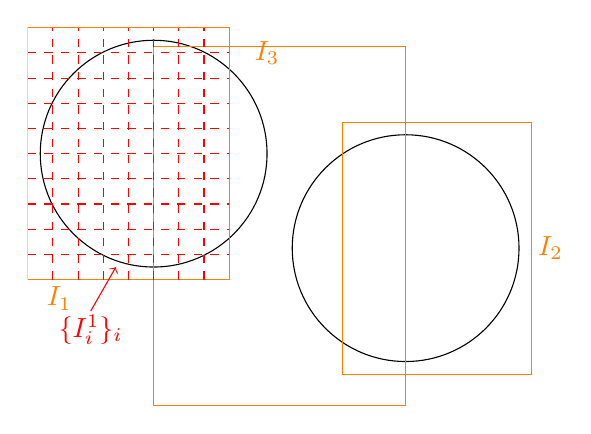
\begin{tikzpicture}[scale=0.8]
                \clip (-2,-4) rectangle (6.5,2);
                \draw (0,0) circle (1.8);
                \draw (4,-1.5) circle (1.8);
                \draw[orange] (-2,-2) rectangle (1.2,2);
                \draw[orange] (0,-4) rectangle (4,1.7);
                \draw[orange] (3,-3.5) rectangle (6,0.5);
                \draw[dashed, red] (-1.6,-2)--(-1.6,2);
                \draw[dashed, red] (-1.2,-2)--(-1.2,2);
                \draw[dashed, red] (-0.8,-2)--(-0.8,2);
                \draw[dashed, red] (-0.4,-2)--(-0.4,2);
                \draw[dashed, red] (0,-2)--(0,2);
                \draw[dashed, red] (0.4,-2)--(0.4,2);
                \draw[dashed, red] (0.8,-2)--(0.8,2);
                \draw[dashed,red] (-2,1.6)--(1.2,1.6);
                \draw[dashed,red] (-2,1.2)--(1.2,1.2);
                \draw[dashed,red] (-2,0.8)--(1.2,0.8);
                \draw[dashed,red] (-2,0.4)--(1.2,0.4);
                \draw[dashed,red] (-2,0)--(1.2,0);
                \draw[dashed,red] (-2,-1.6)--(1.2,-1.6);
                \draw[dashed,red] (-2,-1.2)--(1.2,-1.2);
                \draw[dashed,red] (-2,-0.8)--(1.2,-0.8);
                \draw[dashed,red] (-2,-0.4)--(1.2,-0.4);

                \node[orange] at (-1.5,-2.3) {$I_1$};
                \node[red] at (-1,-2.8) {$\{I_i^1\}_i$};
                \draw[red,->] (-1,-2.5)--(-0.6,-1.8);
                \node[orange] at (6.3,-1.5) {$I_2$};
                \node[orange] at (1.8,1.6) {$I_3$};
            \end{tikzpicture}
        \end{imgbox}
        Siano quindi $H_A =\{h\in H\, |\, J_h\cap A\neq \varnothing\}$ e $H_B =\{h\in H\, |\, J_h\cap B\neq \varnothing\}$. Allora $H_A\cap H_B=\varnothing$, altrimenti esisterebbe un $J_{\bar h}$ tale che $J_{\bar h}\cap A\neq \varnothing$ e $J_{\bar h}\cap B\neq \varnothing$. Ciò implicherebbe che $\operatorname{diam} J_{\bar h}\geq d$, il che è un assurdo per costruzione di $\{J_h\}_h$. Inoltre, per costruzione di $H_A$ e $H_B$, $H_A\cup H_B\subset H$, e quindi $\{J_h\}_{h\in H_A}\in \mc{R}(A)$ e $\{J_h\}_{h\in H_B}\in \mc{R}(B)$. Di conseguenza
        \[\begin{aligned}\mc{L}^n(A)+\mc{L}^n(B) &\leq \sum_{h\in H_A}v(J_h)+\sum_{h\in H_B}v(J_h)=\sum_{h\in H_A\sqcup H_B}\!\!v(J_h) = \substack{\text{ritornando alla}\\\text{notazione precedente}}\\ &= \sum_{j}\sum_{i=1}^{N_j}v(I_i^j)\underset{\eqref{eq: 1.6: 3}}{\leq} \sum_j\left( v(I_j)+\frac{\epsilon}{2^j} \right) = \sum_j v(I_j)+\sum_j\frac{\epsilon}{2^j} \\ & \leq \sum_j v(I_j)+\epsilon \underset{\eqref{eq: 1.6: 2}}< \mc{L}^n(A\cup B) +2\epsilon \end{aligned}\]
        quindi otteniamo 
        \[\mc{L}^n(A)+\mc{L}^n(B) < \mc{L}^n(A\cup B) +2\epsilon \]
        per cui, siccome non vi è dipendenza da $\epsilon$, per $\epsilon\to 0$ si ha la tesi.
        \item \textbf{\underline{Di Radón:}} Poiché $\mc{L}^n$ è metrica, dal Teorema di Carathéodory segue che $\mc{L}^n$ è boreliana (i.e. $\mc{B}(\R^n)\in M_{\mc{L}^n}$)
        \begin{itemize}
            \item \textbf{Borel-regolare:} Sia $A\subset \R^n$ qualsiasi. \hspace{\fill}\boxed{\textsc{tesi: }\exists\, B\in \mc{B}(\R^n)\ :\ B\supset A \;\land\; \mc{L}^n(B)=\mc{L}^n(A)}\\
            Se $\mc{L}^n(A)=+\infty$, la tesi è banale con $X=\R^n$, infatti $B\supset A$, quindi per monotonia $\mc{L}^n(B)\geq \mc{L}^n(A)=+\infty\Rarr \mc{L}^n(B)=+\infty$. Supponiamo quindi $\mc{L}^n(A)<+\infty$.\\
            Di conseguenza $\forall j \exists \{I_i^j\}_i\in \mc{R}(A)$ tale che 
            \[\sum_iv(I_i^j)<\mc{L}^n(A)+\frac{1}{j}<+\infty.\]
            Sia quindi $G_j:=\bigcup_iI_j^i\in \mc{G}$ (NB$^1$: $G_j\supset A$). Ossreviamo che per definizione di $\mc{L}^n$ 
            \begin{equation}\label{eq: 1.6: 4}
                \mc{L}^n(G_j)\leq \sum_iv(I_i^j)\leq \mc{L}^n(A)+\frac{1}{j}
            \end{equation}
            Poniamo infine $B=\bigcap_jG_j\in \mc{B}(R^n)$ (NB$^2$: $B\supset A$, segue da NB$^1$). Scelto allora un qualsiasi $j$,
            \[\mc{L}^n(B)\leq \mc{L}^n(G_j)\underset{\eqref{eq: 1.6: 4}}{\leq} \mc{L}^n(A)+\frac{1}{j}\]
            quindi, per $j\to+\infty$, $\mc{L}^n(B)\leq \mc{L}^n(A)$. Per monotonia di $\mc{L}^n$ e NB$^2$, $\mc{L}^n(A)\leq \mc{L}^n(B)$, da cui la tesi.
            \item \textbf{Di Radón:} 
            Sia $K\in \mc{K}$, allora per il Teorema di Heine-Borel, $K$ è limitato. \hspace{\fill}\boxed{\textsc{tesi: }\mc{L}^n(K)<+\infty}\\
            Allora Esiste un intervallo aperto (N.B. i lati hanno lunghezza finita) $I\subset \R^n$ tale che $K\subset I$, allora $\{I\}\in \mc{R}(K)$. Di conseguenza $\mc{L}^n(K)\leq v(I)=\inf_{\mc{R}(K)}S=S(\{I\})=v(I)<+\infty$.
            \qedhere
        \end{itemize}
    \end{enumerate}
\end{proof}

\begin{definition}
  La misura esterna $\mc{L}^{n}$ definita in Teorema \ref{thm: lebesgue grande} è detta "misura esterna di Lebesgue n-dimensionale".
\end{definition}
Il seguente risultato elenca alcune proprietà della misura esterna di Lebesgue.

\begin{shadedTheorem}[$**$| Lebesgue - piccolo]\label{thm: lebesgue piccolo}
  Valgono i seguenti fatti:
  \begin{enumerate}
      \item Per ogni $a\in \R^n$, si ha $\mc{L}^n(\{a\})=0$;
      \item Se $I$ è un intervallo aperto in $\R^n$, si ha $\mc{L}^n(I)=v(I)$; 
      \item Per ogni $E\in \P(\R^n)\setminus\{\varnothing\}$ e per ogni $\tau\in \R^n$ si ha:
      \begin{enumerate}
          \item $\mc{L}^n(E+\tau)=\mc{L^n}(E)$;
          \item Se $E\in M_{\mc{L}^n}$, allora $E+\tau\in M_{\mc{L}^n}$;
      \end{enumerate}
      \item Per ogni $E\in \P(\R^n)\setminus\{\varnothing\}$ e per ogni $\rho\in\;]0,+\infty[$ si ha:
      \begin{enumerate}
          \item $\mc{L}^n(\rho E)=\rho^n\mc{L}^n(E)$;
          \item Se $E\in M_{\mc{L}^n}$, allora $\rho E\in M_{\mc{L}^n}$;
      \end{enumerate}
  \end{enumerate}
\end{shadedTheorem}
\begin{proof}~
  \begin{enumerate}[label=$(\arabic*)$] 
      \item Sia $a\in \R^n$, sia $\epsilon>0$ arbitrario. \hspace{\fill}\boxed{\textsc{tesi: }\mc{L}^n(\{a\})=0}\\ 
      Sia ora $I_\epsilon = ]-\epsilon, \epsilon[^n+a$ un intervallo aperto contenente $a$. Allora $I_\epsilon\in \mc{R}(\{a\})$, quindi $\mc{L}^n(\{a\}) = \inf_{\mc{R}(\{a\})}S\leq S(\{I_\epsilon\})=v(I_\epsilon)=(2\epsilon)^n$. Poiché $\mc{L}^n(\{a\})$ non dipende da $\epsilon$, per $\epsilon\to 0$ si ha la tesi.
      \item Sia $I$ un intervallo aperto di $\R^n$ qualsiasi.Osserviamo che $\{I\}\in \mc{R}(I)$. \hspace{\fill}\boxed{\textsc{tesi: }\mc{L}^n(I)=v(I)}\\
      Allora $\mc{L}^n(I)=\inf_{\mc{R}(I)}S\leq S(\{I\})=v(I)$, quindi è sufficiente provare la \tesi[ 2]{\mc{L}^n(I)\geq v(I)}

      Siano $\{I_j\}_\in \mc{R}(I)$, $I=]a_1,b_1[\;\times\dots\times\;]a_n,b_n[$. Sia $\varepsilon>0$ sufficientemente piccolo affinché 
      \[J_\varepsilon := [a_1+\varepsilon,b_1-\varepsilon]\;\times\dots\times\;[a_n+\varepsilon,b_n-\varepsilon]\]
      abbia senso (ovvero $\forall i, a_i+\epsilon <b_i-\epsilon$). Allora $J_\epsilon$ è un compatto e $J_\epsilon\subset I\subset \bigcup_jI_j$. Allora per definizione di compattezza, $J_\epsilon$ ammette un sottoricoprimento finito, ovvero $\exists\;\{j_1, \dots, j_n\}\;:\; J_\epsilon^\circ\subset J\epsilon\subset \bigcup_{i=1}^nI_{j_i}$, quindi 
      \[\mc{L}^n(I) = \inf_{\mc{R}(I)}S\geq v(J_\epsilon^\circ)=(b_1-a_1-2\epsilon)\cdot \ldots\cdot (b_n-a_n-2\epsilon)\]
      quindi per $\epsilon \to 0$, $v(J_\epsilon^\circ)\to v(I)$, per cui $\mc{L}^n(I)\geq v(I)$, da cui segue la tesi.

      \item 
      \begin{enumerate}
          \item Sia $E\in\mc{P}(\R^n)\setminus\{\varnothing\}, \tau \in \R^n$. Sia $\{I_j\}_j\in\mc{R}(E)$. \hspace{\fill}\boxed{\textsc{tesi: }\mc{L}^n(E+\tau)=\mc L^n(E)}\\ 
          Allora banalmente $\{I_j+\tau\}_j\in\mc{R}(E+\tau)$.  Inoltre si ha $\forall I,\ v(I)=v(I+\tau)$, quindi 
          \[\mc{L}^n(E+\tau)=\inf_{\mc{R}(E+\tau)}S\leq S(\{I_j+\tau\}_j) = \sum_jv(I_j+\tau)=\sum_jv(I_j)=S(\{I_j\})\]
          quindi, passando all'estremo inferiore, $\mc{L}^n(E+\tau)\leq \mc{L}^n(E)$. Da questo segue che 
          \[\mc{L}^n(E)=\mc{L}^n(E+\tau+(-\tau))\leq \mc{L}^n(E+\tau)\leq \mc{L}^n(E)\ \implies \ \mc{L}^n(E)=\mc{L}^n(E+\tau)\]
          \item Siano $E\in \mc{M}_{\mc{L}^n}$ e $\tau \in \R^n$, $A\in \mc{P}(\R^n)$.  \tesi{E+\tau\in M_{\mc{L}^n}}
          \renewcommand{\arraystretch}{1.8}
          \[\begin{array}{c}
              \mc{L}^n(A\cap(E+\tau))+\mc{L}^n(A\cap \underbrace{(E+\tau)^c}_{E^c+\tau}) = \mc{L}^n(((A-\tau)+\tau)\cap (E+\tau))+ \mc{L}^n(((A-\tau)+\tau)\cap (E^c+\tau))=\\
              =\mc{L}^n(((A-\tau)\cap E)+\tau)+ \mc{L}^n(((A-\tau)\cap E^c)+\tau)=\mc{L}^n((A-\tau)\cap E)+ \mc{L}^n((A-\tau)\cap E^c)=\\
              =\mc{L}^n(A-\tau) = \mc{L}^n(A).
          \end{array}\]
          \renewcommand{\arraystretch}{1}
      \end{enumerate}
      \item 
      \begin{enumerate}
          \item Siano $E\in \mc{P}(R^n)\setminus \{\varnothing\}$, $\rho\in\;]0,+\infty[$. \tesi{\mc{L}^n(\rho E)=\rho^n\mc{L}^n(E)} \\
          Osserviamo che $\forall I$ intervallo, $v(\rho I)=\rho^nv(I)$. Sia $\{I_j\}_j\in \mc{R}(E)$ qualsiasi. Allora $\{\rho I_j\}_j\in \mc{R}(\rho E)$. Di conseguenza 
          \[\mc{L}^n(\rho E)=\inf_{\mc{R}(\rho E)}S\leq S(\{\rho I_j\}_j)=\sum_jv(\rho I_j)=\sum_j\rho^nv(I_j)=\rho^n\sum_jv(I_j)=\rho ^nS(\{I_j\}_j)\]
          quindi passando all'estremo inferiore segue che $\mc{L}^n(\rho E)\leq \rho^n\mc{L}^n(E)$. Da questo segue che
          \[\mc{L}^n(E)=\mc{L}^n(\rho^{-1}\rho E)\leq \rho^{-n}\mc{L}^n(\rho E)\leq \mc{L}^n(E)\ \implies \ \mc{L}^n(\rho E)=\rho^n\mc{L}^n(E)\]
          \item Sia $E\in M_(\mc{L}^n), \rho \in\;]0,+\infty[$. Fissato $A\in \mc{P}(\R^n)$, \tesi{\rho E\in M_{\mc{L}^n}}
          \renewcommand{\arraystretch}{1.8}
          \[\begin{array}{c}
              \mc{L}^n(A\cap \rho E)+\mc{L}^n(A\cap \underbrace{(\rho E)^c}_{\rho E^c}) = \mc{L}^n(\rho\rho^{-1}A \cap \rho E)+\mc{L}^n(\rho \rho^{-1}A \cap \rho E^c)=\\
              = \mc{L}^n (\rho(\rho^{-1}A \cap E))+\mc{L}^n(\rho(\rho^{-1}A\cap E^c)) = \rho^n[\mc{L}^n(\rho^{-1}A\cap E)+\mc{L}^n(\rho^{-1}A\cap E^c)]=\\=\rho^n\mc{L}^n(\rho^{-1}A)=\cancel{\rho^n\rho^{-n}}\mc{L}^n(A).
          \end{array}\]\qedhere
          \renewcommand{\arraystretch}{1}
      \end{enumerate}
  \end{enumerate}
\end{proof}

\begin{exc} Provare le seguenti identità:
  \[
  \begin{gathered}
  (E+\tau)^{c}=E^{c}+\tau, \quad(A+\tau) \cap(B+\tau)=(A \cap B)+\tau \\
  (\rho E)^{c}=\rho E^{c}, \quad(\rho A) \cap(\rho B)=\rho(A \cap B) .
  \end{gathered}
  \]
\end{exc}

\begin{example}Si ha $\mc{L}^{n}\left(\mathbb{Q}^{n}\right)=0$. L'insieme $\mathbb{Q}^{n}$ è misurabile.
\end{example}

\begin{remark} Utilizzando l'insieme di Cantor si può provare che esistono sottoinsiemi di $\mathbb{R}$ che sono misurabili rispetto a $\mc{L}^{1}$ ma non sono Boreliani: sia $\{C_j\}_{j \in \N} \subset \mc{P}(\R^n)$ la successione di insiemi definita ricorsivamente ponendo $C_0 := [0, 1]^n$ e $C_{j+1}$ è l'insieme ottenuto da $C_j$ rimuovendo tutti i terzi medi (aperti) di lunghezza $\sfrac{1}{3^j}$. L'insieme di Cantor è definito quindi come $C := \bigcap_{j \in \N} C_j$. \\
  \begin{tikzpicture}[decoration=Cantor set,very thick]
    
    \draw  (0,0.5) -- (3,0.5);
    \draw decorate{ (0,0) -- (3,0) };
    \draw decorate{ decorate{ (0,-.5) -- (3,-.5) }};
    \draw decorate{ decorate{ decorate{ (0,-1) -- (3,-1) }}};
    \draw decorate{ decorate{ decorate{ decorate{ (0,-1.5) -- (3,-1.5) }}}};
    \node at (-7,-0.5){
      \begin{minipage}{13cm}
        Possiamo osservare innanzitutto che l'insieme di Cantor è ottenuto come intersezione (numerabile) di chiusi, per cui è a sua volta un chiuso. Essendo limitato è inoltre un compatto. Inoltre la successione dei $\{C_j\}$ è decrescente e costituita da misurabili, quindi possiamo applicare il teorema di continuità dall'alto ottenendo che 
        \[\lim_{j\to +\infty} \mc L^1 (C_j) = \mc L^1(C).\]
      \end{minipage}
    };
  \end{tikzpicture}\\
  In particolare, ogni $C^j$ è dato dall'unione disgiunta di $2^j$ segmenti di lunghezza $\sfrac{1}{3^j}$, per cui 
  \[\mc L^1(C) = \lim_{j\to +\infty} \mc L^1 (C_j) = \lim_{j\to +\infty} \left( \frac{2}{3} \right)^j = 0\]
  In particolare, per monotonia $\P(C)\subset \mc M_{\mc L^1}$. 

  Verifichiamo ora che $\operatorname{card}( C )= \operatorname{card}(\R)$: al fine di questa dimostrazione, identifichiamo i numeri reali con il loro allineamento decimale in base 3. Allora l'operazione di rimozione che abbiamo effettuato consiste, al primo passo, a rimuovere tutto ciò che ha 1 come prima cifra decimale, al secondo tutto ciò che ha 1 come seconda cifra decimale e così via. Dobbiamo solo prestare attenzione ai decimali limitati, in quanto quelli che terminano con $1$ sono l'estremo inferiore dei segmenti che stiamo eliminando, e devono rimanere nell'insieme finale: per evitare questo problema è tuttavia sufficiente interpretare $0,1 = 0,0\bar{2}$ e così via. Iterando questo procedimento rimaniamo alla fine con numeri che hanno allineamenti decimali contenenti le sole cifre $0$ e $2$: sostituendo i simboli mediante la legge $0\mapsto 0$ e $2\mapsto 1$ possiamo interpretare questi numeri come allineamenti decimali in base 2 e osservare che in questo modo stiamo riscrivendo in un'altra base lo stesso intervallo $[0,1]$.

  Come diretta conseguenza di questa trattazione abbiamo quindi che 
  \[
  \operatorname{card}(\mathbb{R})=\operatorname{card}(C)<\operatorname{card}\left(\P({C})\right) \leq \operatorname{card}\left(\mc{M}_{\mc{L}^{1}}\right)
  \]
  A questo punto la conclusione segue subito dal fatto che $\operatorname{card}(\mc{B}(\mathbb{R}))=\operatorname{card}(\mathbb{R})$, per la dimostrazione del quale rimandiamo a $[\mathbf{1 5}]$.
\end{remark}
\begin{example}[Esistenza di insiemi non misurabili: l'esempio di Vitali] Consideriamo la seguente relazione di equivalenza in $[0,1]: x \sim y$ se $x-y \in \mathbb{Q}$. Grazie all'assioma della scelta possiamo poi "costruire" un insieme $E\subset [0,1]$ di rappresentanti delle classi di equivalenza. Se $\mathbb{Q} \cap\ [-1,1]=\left\{q_{i}\right\}_{i \in \mathbb{N}}$, poniamo infine $E_j = E + q_j$: allora $\mc L^1(E_j) = \mc L^1(E)$ e $\forall j, E_j\subset [-1,2]$. 
\begin{itemize}
  \item Verifichiamo inizialmente che $[0,1]\subset \bigcup_jE_j$: fissato $x\in [0,1]$, deve esistere un $e\in E$ tale che $x-e\in \Q$ (in particolare, poiché $x,e\in [0,1]$, $x-e\in [-1,1]$). Di conseguenza deve esistere un $j$ tale che $x-e = q_j$, per cui $x = e+q_j\in E+q_j = E_j$.
  \item Osserviamo quindi che gli $\{E_j\}_j$ sono a-2-a-2 disgiunti: siano infatti $i\neq j$, supponiamo per assurdo che esista $x\in E_i\cap E_j$. Si avrebbe quindi $x = e_1+q_i = e_2+q_j$ con $e_1,e_2\in E$, da cui $e_1-e_2 = q_j-q_i\in \Q$. Questo implicherebbe $e_1\sim e_2$, ovvero $e_1 = e_2$ per costruzione di $E$, da cui $q_i = q_j$ e $i = j$, assurdo.
\end{itemize}
Proviamo infine che $E$ non è misurabile: supponiamo per assurdo che lo sia, allora per il Piccolo Teorema di Lebesgue tutti gli $E_j$ avrebbero la sua stessa misura, da cui 
\[\textstyle 1 = \mc L^1([0,1]) \leq \mc L^1( \bigcup_jE_j)\leq \mc L^1([-1,2]) = 3.\tag{$*$}\]
In particolare, per $\sigma$-additività, avremmo 
\[\textstyle \mc L^1( \bigcup_jE_j) = \sum_j\mc L^1(E_j) = \sum_j\mc L^1(E).\]
A questo punto si configurano due casi: se $L^1(E) = 0$, la serie ha somma nulla (quando per ($*$) dovrebbe essere maggiore di $1$); se $L^1(E)>0$ la serie diverge in quanto la successione degli addendi e positiva e non infinitesma (quando per $(*)$ dovrebbe essere limitata). In entrambe le situazioni si configura un assurdo, per cui $E$ non può essere misurabile.
\end{example}
\begin{exc}[\footnote{Già incluso nell'Esempio, NdR}]Provare che se $i \neq j$ allora $E_{i} \cap E_{j}=\varnothing$.
\end{exc}
\begin{remark}Senza l'assioma della scelta è impossibile provare l'esistenza di insiemi non misurabili (Solovay, 1970).\end{remark}

\subsection{Misura esterna di Hausdorff}
\begin{shadedTheorem}[$*$| Premisura di Hausdorff]\label{thm: 1.8 premisura Hausdorff}
  Dati $E\in\P(\R^n)$ e $\delta >0$, indichiamo con $\mc R_\delta (E)$ la famiglia dai ricoprimenti numerabili $\{C_j\}_j$ di $E$ tali che $0<\operatorname{diam}C_j\leq \delta$ $\forall j$. Per $s\in [0,+\infty[$, poniamo anche 
  \[\alpha(s):=\frac{\pi^{s/2}}{\Gamma\left(\frac{s}{2}+1\right)},\qquad \Gamma(t):=\int_0^{+\infty} e^{-x}x^{t-1}\operatorname{d}\!x.\]
  Allora la funzione $\mc{H}^s_\delta:\P(\R^n)\to [0,+\infty]$ definita da
  \[\mc{H}^s_\delta(E):=\begin{cases}
       \inf\left\{\sum_j\alpha(s)\left( \frac{\operatorname{diam}C_j}{2} \right)^s\,\Big|\,\{C_j\}_j\in\mc{R}_\delta (E)\right\} & \text{ se } E\neq \varnothing\\
       0 & \text{ se } E = \varnothing
   \end{cases}\]
   è una misura esterna
\end{shadedTheorem}

\begin{remark}Si può provare che $\alpha(n)=\mc{L}^{n}\left(B_{1}^{(n)}\right)$, dove $B_{1}^{(n)}$ è la palla unitaria di $\mathbb{R}^{n}$. Per una dimostrazione di questo fatto, si veda per esempio [16, Ch. 2, Exercise 14].
\end{remark}

\begin{proof}Verifichiamo gli assiomi di misura esterna:
  \begin{enumerate}[label=$\roman*)$]
      \item Il primo assioma di misura esterna ($\mc H_\delta^s(\varnothing) = 0$) è verificato per definizione.
      \item Siano $E \subset F \subset \R^n$, vogliamo dimostrare che $\mc H_\delta^s(E) \le \mc H_\delta^s(F)$.\\
          Se $E = \varnothing$ è banale, altrimenti $\mc R_\delta(E) \supset \mc R_\delta(F)$, dunque $\inf_{\mc R_\delta(E)} S \le \inf_{\mc R_\delta(F)} S$ e perciò $\mc H_\delta^s(E) \le \mc H_\delta^s(F)$.
      \item Sia $\{E_j\}_{j \in J} \subset \mc P(\R^n)$ numerabile, vogliamo dimostrare la $\sigma$-subaddittività.\\
          Se $\sum_{j \in J} \mc H_\delta^s(E_j) = + \infty$ la tesi è banale, come nel caso in cui $\bigcup_{j \in J} E_j = \varnothing$, supponiamo dunque che la somma sia finita e la famiglia non vuota con almeno un insieme non vuoto.\\
          Sia $J^* := \{ j \in J | E_j \neq \varnothing\}$ che per ipotesi è non vuoto, la nostra nuova tesi diventa $\mc H_\delta^s(\bigcup_{j \in J^*} E_j) \le \sum_{j \in J^*} \mc H_\delta^s(E_j)$, somma che abbiamo già assunto finita (e perciò la misura di ogni singolo insieme nella famiglia è finita).\\
          Di conseguenza, fissato $\varepsilon > 0$, abbiamo che $\forall j \in J^*, \exists \{C_i^j\}_{i \in I_j} \in \mc R_\delta(E_j)$ tale che \[S(\{C_i^j\}_{i \in I_j}) \le \mc H_\delta^s(E_j) + \frac{\varepsilon}{2^j}.\]\\
          Osserviamo quindi che $\{C_i^j\}_{i \in I_j,j \in J^*} \in \mc R_\delta(\bigcup_{j \in J^*} E_j)$ e perciò \[\mc H_\delta^s\bigg(\bigcup_{j \in J^*} E_j\bigg) \le S(\{C_i^j\}_{i \in I_j, j \in J^*}) = \sum_{j \in J^*} S(\{C_i^j\}_{i \in I_j}) \le \varepsilon + \sum_{j \in J^*} \mc H_\delta^s(E_j).\]\\
          Quini, per $\epsilon \to 0$, si ha la tesi.
  \end{enumerate}        
\end{proof}

\begin{exc}Verificare col calcolo diretto che: $\alpha(0)=1, \quad \alpha(1)=2, \quad \alpha(2)=\pi, \quad \alpha(3)=\frac{4 \pi}{3}$.\end{exc}

\begin{shadedTheorem}[$**$| Hausdorff]\label{thm: 1.9 Hausdorff}
  Sia $s\in [0,+\infty[$ e $E\in \P(\R^n)$. Allora la funzione $\delta \mapsto \mc{H}^s_\delta(E)$ è monotona decrescente, quindi esiste 
  \[\mc{H}^s(E)=\lim_{\delta \to 0}\mc{H}^s_\delta(E).\]
  La mappa $\mc{H}^s:\P(\R^n)\to [0,+\infty]$ è una misura esterna metrica e Borel regolare. Essa è detta \say{misura di Hausdorff $s$-dimensionale $($in $\R^n)$}.
\end{shadedTheorem}
\begin{proof}~
  \begin{enumerate}[label=\textbf{\Large\arabic*.}, ref=\textbf{\underline{(\arabic*)}}]
      \item \textbf{\underline{Monotonia}:} Siano $\delta_1, \delta_2 \in \R \ :\  0<\delta_1 < \delta_2$. Vogliamo dimostrare che $\mc H_{\delta_1}^s(E) \le \mc H_{\delta_2}^s(E)$.\\
      Osserviamo che $\mc R_{\delta_1}(E) \supset \mc R_{\delta_2}(E)$, dunque $\inf_{\mc R_{\delta_1}(E)}S \le \inf_{\mc R_{\delta_2}(E)}S$, ovvero la tesi. Di conseguenza, per il teorema di esistenza di limite per funzioni monotone, esiste $\mc{H}^s_\delta(E)$.
      \item \textbf{\underline{Misura esterna}:} \begin{enumerate}[label=$\roman*)$]
          \item $\mc{H}^s(\varnothing)=\lim\limits_{\delta \to 0}\mc{H}^s_\delta(\varnothing)=\lim\limits_{\delta \to 0}0=0$;
          \item Siano $E,F\in \mc{P}(\R^n),\ E\subset S$. Allora $\forall \delta, \mc{H}^s_\delta(E)\leq \mc{H}^s_\delta(F)$, per cui facendo tendere $\delta$ a $0$, si ha $\mc{H}^s(E)\leq \mc{H}^s(F)$;
      \end{enumerate}
      N.B. Poiché $\mc{H}^s(E)=\lim\limits_{\delta \to 0}\mc{H}^s_\delta(E)$ e la funzione $\delta \mapsto \mc{H}^s_\delta(E)$ è decrescente, segue che $\forall \delta\ \mc{H}^s_\delta(E)\leq \mc{H}^s(E)$.
      \begin{enumerate}[resume,label=$\roman*)$]
          \item Sia $\{E_j\}_{j}$ numerabile. \tesi{\mc{H}^s\Bigl(\bigcup\nolimits_jE_j\Bigr)\leq \sum\nolimits_j\mc{H}^s(E_j)}\\
          Poiché $\mc{H}^s_\delta$ è una misura esterna si ha \[\mc{H}^s_\delta\Bigl(\bigcup\nolimits_jE_j\Bigr)\leq \sum\nolimits_j\mc{H}^s_\delta(E_j)\leq \sum\nolimits_j\mc{H}^s(E_j)\quad \forall \delta >0\]
          \[\underset{\delta \to 0}\implies \mc{H}^s\Bigl(\bigcup\nolimits_jE_j\Bigr) = \lim_{\delta \to 0}\mc{H}^s_\delta\Bigl(\bigcup\nolimits_jE_j\Bigr)\leq \sum\nolimits_j\mc{H}^s(E_j)\]
      \end{enumerate}
      \item \textbf{\underline{Metrica}:} Siano $A,B\in \mc{P}(\R)$ tali che $\operatorname{dist}(A,B)=d>0$. Poiché vale la $\sigma$-subadditività, è sufficiente provare la \tesi{\mc{H}^s(A\cup B)\geq\mc{H}^s(A)+\mc{H}^s(B)}\\
      Se $\mc{H}^s(A\cup B)=+\infty$, la tesi è banale. Supponiamo quindi $\mc{H}^s(A\cup B)<+\infty$. Allora per quanto detto precedentemente, anche $\mc{H}^s_\delta(A\cup B)<+\infty$. Proviamo innanzitutto che $\forall \delta <d$ si ha \[\mc{H}^s_\delta(A\cup B)\geq \mc{H}^s_\delta(A)+\mc{H}^s_\delta(B)\]
      Siano $\delta < d$ e $\epsilon >0$. Poiché
      $+\infty>\mc{H}^s_\delta(A\cup B)=\inf_{\mc{R}_\delta(A\cup B)}S$, esiste una famiglia $ \{C_j\}_j\in\mc{R}_\delta(A\cup B)$ tali che $S(\{C_j\}_j)<\mc{H}^s_\delta(A\cup B)+\epsilon\ \ (*)$. Per costruzione si ha quindi che $\forall j,$ $C_j$ non interseca sia $A$ che $B$. Definiamo $J_A:=\{j\in J\,|\,C_j\cap A\neq \varnothing\}$ e osserviamo che $J_A\neq \varnothing$ e $\{C_j\}_{j\in \A}\in \mc{R}_\delta (A)$; analogamente per $J_B$. Osserviamo inoltre che $J_A\sqcup J_B\subset J$, quindi 
      \[\begin{aligned}\mc{H}^s_\delta(A)+\mc{H}^s_\delta(B)&\leq S(\{C_j\}_{j\in J_A})+S(\{C_j\}_{j\in J_B})= \sum_{j\in J_A}\alpha(s)\left( \frac{\operatorname{diam}C_j}{2} \right)^s+\sum_{j\in J_B}\alpha(s)\left( \frac{\operatorname{diam}C_j}{2} \right)^s=\\&=\sum_{j\in J_A\sqcup J_B}\alpha(s)\left( \frac{\operatorname{diam}C_j}{2} \right)^s\leq \sum_{j\in J}\alpha(s)\left( \frac{\operatorname{diam}C_j}{2} \right)^s=S(\{C_j\}_{j\in J})\underset{(*)}<\mc{H}^s_\delta(A\cup B)+\epsilon\end{aligned}\] 
      per cui, per $\epsilon \to 0$, si ha che $\mc{H}^s_\delta(A\cup B)\geq \mc{H}^s_\delta(A)+\mc{H}^s_\delta(B)$. Passando al limite per $\delta \to 0$, segue la tesi. 
      \item \textbf{\underline{Borel-Regolare}:} Poiché $\mc{H}^s$ è metrica, per il teorema di Carathéodory segue che $\mc{H}^s$ è boreliana. Rimane da provare la Borel-regolarità: sia $A\in \mc{P}(X)$. \tesi{\exists B\in \mc{B}(X)\ :\ B\supset A\ \land\ \mc{H}^s(A)=\mc{H}^s(B)}\\
      Se $\mc{H}^s(A)=+\infty$, basta prendere $B=\R^n$. Allora $B=\R^n\supset A$ e $\mc{H}^s(\R^n)=+\infty$ per monotonia. Supponiamo quindi $\mc{H}^s_\delta(A)<+\infty$. Allora per ogni $j\in \Z^+, \mc{H}^s_\frac{1}{j}(A)\leq \mc{H}^s(A)<+\infty$. Conseguentemente, esiste una famiglia $\{C_i^j\}_{i\in I_j}\in \mc{R}_{\frac{1}{j}}(A)$ tale che
      \[S(\{C^j_i\}_{i\in I_j})<\mc{H}^s_\frac{1}{j}(A)+\frac{1}{j} \tag{$**$}\]
      dove $S(\{C^j_i\}_{i\in I_j}) = \sum_{i\in I_j}\alpha(s)\left(\frac{\operatorname{diam}C^j_i}{2}\right)^s=\sum_{i\in I_j}\alpha(s)\left(\frac{\operatorname{diam}\bar C^j_i}{2}\right)^s$  in quanto $\operatorname{diam}C = \operatorname{diam}\bar C$. Consideriamo ora $B_j=\bigcup_{i\in I_j}\bar C^j_i\in \mc{B}(\R^n)$ in quanto tutti i $C^j_i$ sono chiusi. Poiché $\{C_i^j\}_{i}\in \mc{R}_\frac{1}{j}(A)$, allora $A\subset \bigcup_i C_i^j\subset \bigcup \bar C_j^i \subset B_j$. 

      Abbiamo quindi $B\supset A$. Rimane quindi da provare l'uguaglianza delle misure di Hausdorff. Per monotonia vale già un verso della disuguaglianza, rimane pertanto da provare la \tesi[ 2]{\mc{H}^s(B)\leq \mc{H}^s(A)}\\
      Abbiamo quindi che 
      \[\mc{H}^s_{\frac{1}{j}}(B)\underset{(\bullet)}\leq\sum_j\alpha(s)\left( \frac{\operatorname{diam}\bar C_i^j}{2}\right)^s\underset{(**)}\leq \mc{H}^s_\frac{1}{j}(S)+\frac{1}{j}\]
      (\textbullet) in quanto $\{\bar C_i^j\}\in \mc{R}_\frac{1}{j}(B_j)$. Di conseguenza, per $j\to +\infty$, segue la tesi.\qedhere
  \end{enumerate}
\end{proof}

\begin{exc}Provare che se $X$ è uno spazio metrico, allora per ogni sottoinsieme $C$ di $X$ si ha $\operatorname{diam} C=\operatorname{diam} \bar{C}$. 
\end{exc}

Alcune ulteriori proprietà della misura esterna di Hausdorff sono raccolte in questo teorema di cui non proviamo il punto (2) e lasciamo per esercizio le parti dei punti (3) e (4) che replicano quasi identicamente gli argomenti usati per provare le corrispondenti asserzioni in Teorema \ref{thm: lebesgue piccolo}. La dimostrazione del punto (2) è un argomento (basato sulla disuguaglianza isodiametrica) che non abbiamo tempo di affrontare. Gli interessati possono consultare, per esempio, $[\mathbf{3}, \mathbf{11}]$.


\begin{shadedTheorem}[$*$| Hausdorff - piccolo]\label{thm: hausdorff piccolo}
  Si ha:
  \begin{enumerate}
    \item $\mc{H}^{0}=\#$ (misura del conteggio);
    \item $\mc{H}^{n}=\mc{L}^{n}\left(\right.$in $\left.\mathbb{R}^{n}\right)$ - non lo dimostriamo;
    \item Per ogni insieme non vuoto $E \subset \mathbb{R}^{n}$ e per ogni $\tau \in \mathbb{R}^{n}$ si ha:
    \begin{itemize}
      \item $\mc{H}^{s}(E+\tau)=\mc{H}^{s}(E)$
      \item Se $E \in \mc{M}_{\mc{H}^{s}}$ allora $E+\tau \in \mc{M}_{\mc{H}^{s}}$;
    \end{itemize}
    \item Per ogni insieme non vuoto $E \subset \mathbb{R}^{n}$ e per ogni $\rho \in \mathbb{R}^{+}$si ha:
    \begin{itemize}
      \item $\mc{H}^{s}(\rho E)=\rho^{s} \mc{H}^{s}(E)$;
      \item Se $E \in \mc{M}_{\mc{H}^{s}}$ allora $\rho E \in \mc{M}_{\mc{H}^{s}}$;
    \end{itemize}
  \end{enumerate}
\end{shadedTheorem}
\begin{proof}~
  \begin{enumerate}
      \item \begin{itemize}
          \item Se $E = \varnothing$, la tesi segue banalmente.
          \item Se $E = \{p\} \in \R^n$, si ha che $\forall \delta > 0$ vale \[\mc H_\delta^0(E) = \inf\left\{\left.\sum_j \alpha(0)\left(\frac{\operatorname{diam}(C_j)}{2}\right)^0\right|\{C_j\}_j \in \mc R_\delta(E)\right\} = \inf\{\#\{C_j\}_j |\{C_j\}_j \in \mc R_\delta(E)\}\] Dato che $E \neq \varnothing$ abbiamo $\forall \{C_j\}_j \in \mc R_\delta(E),\#\{C_j\}_j \geq 1$, quindi $\mc H_\delta^0(E) \geq 1$.\\ Inoltre, $\operatorname{diam}(B_{\delta/3}(p)) = \frac{2\delta}{3}<\delta \Rarr B_{\delta/3}(p) \in \mc R_\delta(E)$, dunque $1 \leq \mc H_\delta^0(E) \leq S(B_{\delta/3}(p)) \leq 1 \Rarr \forall \delta > 0 , \mc H_\delta^0(E) = 1 \Rarr \mc H^0(E) = 1$.
          \item Sia $E$ finito. Allora $E = \bigcup_j \{p_j\}$ con $\forall i \neq j, d(p_i,p_j) > 0$ e dal teorema di \textbf{\textit{Carathéodory}} segue $\mc H^0 (E) = \sum_j \mc H(p_j) = \sum_j 1 = \#E$.
          \item Sia $E$ un insieme infinito. Allora $\forall N > 0, \exists F \subset E | \#F = N \Rarr \mc H^0(E) > \mc H^0(F)=\#F=N \Rarr \mc H^0(E) = +\infty$.
      \end{itemize}
      \item La dimostrazione del secondo punto viene omessa.
      \item Sia $E \in \mc P(\R^n)$ e $\tau \in \R^n$. \\ Posto $\delta > 0$ si ha $\{C_j\}_j \in \mc R_\delta(E) \Rarr \{C_j+\tau\}_j \in \mc R_\delta(E+\tau)$ dunque \[\mc H_\delta^s(E+\tau) = \inf_{\mc R_\delta(E+\tau)}S \leq S(\{C_j+\tau\}_j) = S(\{C_j\}_j) \Rarr \mc H_\delta^s(E+\tau) \leq \mc H_\delta^s(E)\]. Ora, $\mc H_\delta^s(E) = \mc H_\delta^s((E+\tau)-\tau) \leq \mc H_\delta^s(E+\tau)$, dunque $\forall \delta > 0, \mc H_\delta^s(E)=\mc H_\delta^s(E+\tau)\Rarr \mc H^s(E+\tau) = \mc H^s(E+\tau)$. \\ La dimostrazione del secondo punto di questo terzo punto è  analoga a quella per la misura di Lebesgue (Teorema \ref{thm: lebesgue piccolo}).
      \item Sia $\varnothing \neq E \in \mc P(\R^n)$ e siano $\rho ,\delta \in ]0,+\infty[$. Si ha che $\{C_j\}_j \in \mc R_\delta(E) \Rarr \{\rho C_j\}_j \in \mc R_{\rho \delta}(\rho E)$ e quindi \[\mc H_{\rho \delta}^s(\rho E) \leq S(\{\rho C_j\}_j) = \rho ^sS(\{C_j\}_j) \Rarr \mc H_{\rho \delta}^s(\rho E) \leq \rho ^s \mc H_{\delta}^s(E)\] Abbiamo anche \[\mc H_{\delta}^s(E) = \mc H_{\frac{1}{\rho }\rho \delta}^s(E) \leq \frac{1}{\rho ^s}\mc H_{\rho \delta}^s(\rho E)\] E quindi $\mc H_{\rho \delta}^s(\rho E) = \rho ^s\mc H_{\delta}^s(E)$. Mandando $\delta$ a $0$ segue la tesi. \\ La dimostrazione del secondo punto di questo quarto punto è  analoga a quella per la misura di Lebesgue (Teorema \ref{thm: lebesgue piccolo}).
  \end{enumerate}
\end{proof}

\begin{exc}Relativamente a Teorema \ref{thm: hausdorff piccolo}:

\begin{itemize}
  \item Provare che, per ogni $C \subset \mathbb{R}^{n}$ e per ogni $\rho \in \mathbb{R}^{+}$, si ha $\operatorname{diam}(\rho C)=\rho \operatorname{diam}(C)$;

  \item Provare il secondo punto di (3) ed il secondo punto di (4).
\end{itemize}
\end{exc}
\noindent Attraverso le proprietà della misura di Hausdorff si può definire una nozione di dimensione per i sottoinsiemi di $\mathbb{R}^{n}$.

\begin{proposition}[$*$]\label{prop: 1.4 dimensione Hausdorff} Se $\mc{H}^{s}(E)<+\infty$, con $E \subset \mathbb{R}^{n}$ e $s \geq 0$, allora $\mc{H}^{t}(E)=0$ per ogni $t>s$. Inoltre, per ogni $t>n$ si ha $\mc{H}^{t}\left(\mathbb{R}^{n}\right)=0$. Conseguentemente, per ogni $E \subset \mathbb{R}^{n}$, l'insieme
\[
R(E):=\left\{t \in[0,+\infty) \mid \mc{H}^{t}(E)=0\right\}
\]
è una semiretta destra che include $(n,+\infty)$. La "dimensione di Hausdorff" dell'insieme $E \subset \mathbb{R}^{n}$ è definita come il numero
\[
\operatorname{dim}_{H}(E):=\inf R(E) \leq n
\]
\end{proposition}
\begin{proof}
  \begin{itemize}
      \item Siano $E \in \mc P(\R^n), s \in [0,+\infty[$ tali che $\mc H^s(E) < +\infty$ e sia $t>s$. Per la dimostrazione precedente, con $\delta > 0$ si ha $\mc H_{\delta}^s(E) \leq \mc H^s(E) < +\infty$, dunque $\exists \{C_j\}_j \in \mc R_\delta(E):$ \[\sum_j \alpha(s) \left(\frac{\operatorname{diam}(C_j)}{2}\right)^s < \mc H_{\delta}^s(E) +1 \leq \mc H^s(E) + 1 < +\infty\]. Allora si ha 
      \[\begin{aligned}\mc H_{\delta}^t(E) &\leq \sum_j \alpha(t) \left(\frac{\operatorname{diam}(C_j)}{2}\right)^t = \frac{\alpha(t)}{\alpha(s)}\sum_j \alpha(s) \left(\frac{\operatorname{diam}(C_j)}{2}\right)^s \left(\frac{\operatorname{diam}(C_j)}{2}\right)^{t-s} \leq \\ &\leq\frac{\alpha(t)}{\alpha(s)} \left(\frac{\delta}{2}\right)^{t-s}\sum_j \alpha(s) \left(\frac{\operatorname{diam}(C_j)}{2}\right)^s \leq  \frac{\alpha(t)}{\alpha(s)} \left(\frac{\delta}{2}\right)^{t-s} (\mc H^s(E) + 1)\end{aligned}\] Dunque mandando $\delta$ a $0$ otteniamo $\mc H^t(E) \leq 0 \Rarr \mc H^t(E) = 0$.
      \item Sia $t>n$. Osserviamo che $\R^n = \bigcup_{j=0}^{+\infty} B_j(0)$ e ovviamente $\mc H^n (B_j(0)) = \mc L^n(B_j(0)) = \mc L^n(\bar{B}_j(0)) < +\infty$, dunque la $\forall j \in \N, \mc H^t(B_j(0)) = 0$ e per la $\sigma$-subadditività della misura di Hausdorff si ha $\mc H^t(\R^n) = 0$ 
      \item Sia $E \in \mc P(\R^n)$ e siano $s \in R(E)$ e $t>s$. Per quanto appena detto, $\mc H^t(E) = 0$, dunque $t \in R(E)$.
      \item Sia $t > n$, allora $t \in R(\R^n) \Rarr \forall E \in \mc P(\R^n), t \in R(E)$.
      \item Dai punti seguenti segue che $n = \inf]n,+\infty[ \geq \inf R(E) = \dim_{\mc H} E$
  \end{itemize}
\end{proof}

\begin{corollary}[$*$]\label{cor: 1.2 Hausdorff non Radon}
  La misura esterna di Haudorff $\mc{H}^{s}$ in $\mathbb{R}^{n}$ non è di Radón, eccetto che per $s \geq n$.
\end{corollary}
\begin{proof}~
  \begin{enumerate}[label=$(\roman*)$]
    \item $\mc{H}^s$ è di Radón in quanto coincide con $\mc{L}^n$.
    \item Se $t>n$, $\mc{H}^t$ è di Radón in quanto $\mc{H}^t(\R^n)=0$, quindi per monotonia $\mc{H}^t(E)=0\ \forall E\in \P(\R^n)$.
    \item Sia $s<n$, verifichiamo che $\mc{H}^s$ non è di Radón fornendo un controesempio: supponiamo per assurdo che $\mc{H}^s([0,1])<+\infty$, allora per la proposizione precedente $\mc{H}^n([0,1]^n)=0$, quindi $0=\mc{H}^n([0,1]^n)=\mc{L}^n([0,1]^n)=1$. Assurdo.\qedhere
  \end{enumerate}
\end{proof}

\begin{example}Sia $C$ l'insieme di Cantor. Non è facile verificare che esiste $s$ tale che $\mc{H}^{s}(C) \in]0,+\infty[$, ma se proviamo a supporre che esista allora troviamo facilmente che deve essere $s=\operatorname{dim}_{H}(C)=\sfrac{\ln 2}{\ln 3}$. Questo ci consente di "scommettere" che $C$ abbia effettivamente dimensione di Hausdorff pari a $\ln 2 / \ln 3$.\\
Osserviamo inizialmente che $C_2 = (\sfrac{1}{3}C_1)\cup (\sfrac{1}{3}C_1+\sfrac{2}{3})$ e che, in generale, $C_{k+1} = (\sfrac{1}{3}C_k)\cup (\sfrac{1}{3}C_k+\sfrac{2}{3})$. Questo ci porta a scrivere quindi la relazione $C = (\sfrac{1}{3}C)\cup (\sfrac{1}{3}C+\sfrac{2}{3})$, dove $\sfrac{1}{3}C$ e $\sfrac{1}{3}C+\sfrac{2}{3}$ sono insiemi a distanza positiva. In particolare, ricordando che $\mc H^s$ è metrica e supponendo (non è detto che ciò sia vero, lo proveremo successivamente) che esista un $s$ tale per cui $\mc H^s(C)\in\ ]0,+\infty[$,
\[\mc H^s(C) = \mc H^s\left(\frac{1}{3}C\right)+\mc H^s\left(\frac{1}{3}C+\frac{2}{3}\right) = 2 \left(\frac{1}{3}\right)^s \mc H^s(C).\]
Siccome abbiamo supposto $\mc H^s(C)\neq 0$, possiamo dividere, ottenendo 
\[1 = \frac{2}{3^s} \implies s = \frac{\ln 2}{\ln 3}.\]
Se tale $s$ esiste, quindi, vale $\sfrac{\ln 2}{\ln 3}$: rimane da provare che effettivamente le ipotesi che abbiamo fatto sono giustificate, ovvero che $\mc H^s(C) \in\ ]0,+\infty[$. Calcolando la misura di Hausdorff dell'insieme di Cantor, otteniamo infatti 
\[\mc H^{\frac{\ln 2}{\ln 3}} (C) = \alpha\left(\frac{\ln 2}{\ln 3}\right)\]
per cui la misura di Hausdorff di $C$ è effettivamente $\operatorname{dim}_{H}(C)=\sfrac{\ln 2}{\ln 3}$.\\
Per una dimostrazione più completa si faccia riferimento, per esempio, a [4, Theorem 1.14] oppure a [16, Ch. 7, Theorem 2.1].
\end{example}

\begin{definition}[Misura]Sia $X$ un insieme e $\mc{A}$ una $\sigma$-algebra in $X$. Allora, una "misura su $\mc{A}$ " è una funzione $\mu: \mc{A} \rightarrow[0,+\infty]$ tale che:
  \begin{enumerate}[label=$(\roman*)$]
    \item $\mu(\varnothing)=0$;
    \item se $\left\{E_{j}\right\}$ è una famiglia numerabile di insiemi in $\mc{A}$ a-due-a-due disgiunti, allora $\mu\left(\cup_{j} E_{j}\right)=\sum_{j} \mu\left(E_{j}\right)$.
  \end{enumerate}
  La terna $(X, \mc{A}, \mu)$ è detta "spazio con misura".
\end{definition}
Come conseguenza di Teorema \ref{thm: proprietà misurabili} e Proposizione \ref{prop: misurabili sigma-algebra}, otteniamo subito il seguente risultato.

\begin{proposition}[$\circ$] \label{prop: misura esterna è misura}Se $\varphi$ è una misura esterna sull'insieme $X$, allora $\left(X, \mc{M}_{\varphi},\left.\varphi\right|_{\mc{M}_{\varphi}}\right)$ è uno spazio con misura.
\end{proposition}
\begin{proof}~
  \begin{enumerate}[label=$(\roman*)$]
    \item $\phi(\varnothing)=0$ per assioma di misura esterna;
    \item se $\left\{E_{j}\right\}$ è una famiglia numerabile di insiemi in $\mc{M}_\phi$ a-due-a-due disgiunti, allora $\phi\left(\cup_{j} E_{j}\right)=\sum_{j} \mu\left(E_{j}\right)$ per il Teorema \ref{thm: proprietà misurabili}.
  \end{enumerate}
\end{proof}

\begin{example}La "misura di Lebesgue" $\left.\mc{L}^{n}\right|_{\mc{M}_{\mc{L}^{n}}}$ e la "misura di Hausdorff" $\left.\mc{H}^{s}\right|_{\mc{M}_{\mc{H}^{s}}}$. Per semplicità esse sono indicate con $\mc{L}^{n}$ and $\mc{H}^{s}$, rispettivamente.
\end{example}

\begin{remark}Ci si può chiedere se una misura provenga sempre da una misura esterna nel modo indicato in Proposizione \ref{prop: misura esterna è misura}. Una risposta quasi affermativa è data dal seguente risultato (vedasi [5, Theorem 4.47]): 
\end{remark}

\begin{shadedTheorem}
  Se $(X, \mc{A}, \mu)$ è uno spazio con misura, allora esiste una misura esterna $\varphi$ su $X$ tale che $\mc{A} \subset \mc{M}_{\varphi}$ e $\left.\varphi\right|_{\mc{A}}=\mu$.
\end{shadedTheorem}


